% Options for packages loaded elsewhere
% Options for packages loaded elsewhere
\PassOptionsToPackage{unicode}{hyperref}
\PassOptionsToPackage{hyphens}{url}
\PassOptionsToPackage{dvipsnames,svgnames,x11names}{xcolor}
%
\documentclass[
doublespace,
  times]{anzsauth}
\usepackage{xcolor}
\usepackage{amsmath,amssymb}
\setcounter{secnumdepth}{5}
\usepackage{iftex}
\ifPDFTeX
  \usepackage[T1]{fontenc}
  \usepackage[utf8]{inputenc}
  \usepackage{textcomp} % provide euro and other symbols
\else % if luatex or xetex
  \usepackage{unicode-math} % this also loads fontspec
  \defaultfontfeatures{Scale=MatchLowercase}
  \defaultfontfeatures[\rmfamily]{Ligatures=TeX,Scale=1}
\fi
\usepackage{lmodern}
\ifPDFTeX\else
  % xetex/luatex font selection
\fi
% Use upquote if available, for straight quotes in verbatim environments
\IfFileExists{upquote.sty}{\usepackage{upquote}}{}
\IfFileExists{microtype.sty}{% use microtype if available
  \usepackage[]{microtype}
  \UseMicrotypeSet[protrusion]{basicmath} % disable protrusion for tt fonts
}{}
\makeatletter
\@ifundefined{KOMAClassName}{% if non-KOMA class
  \IfFileExists{parskip.sty}{%
    \usepackage{parskip}
  }{% else
    \setlength{\parindent}{0pt}
    \setlength{\parskip}{6pt plus 2pt minus 1pt}}
}{% if KOMA class
  \KOMAoptions{parskip=half}}
\makeatother
% Make \paragraph and \subparagraph free-standing
\makeatletter
\ifx\paragraph\undefined\else
  \let\oldparagraph\paragraph
  \renewcommand{\paragraph}{
    \@ifstar
      \xxxParagraphStar
      \xxxParagraphNoStar
  }
  \newcommand{\xxxParagraphStar}[1]{\oldparagraph*{#1}\mbox{}}
  \newcommand{\xxxParagraphNoStar}[1]{\oldparagraph{#1}\mbox{}}
\fi
\ifx\subparagraph\undefined\else
  \let\oldsubparagraph\subparagraph
  \renewcommand{\subparagraph}{
    \@ifstar
      \xxxSubParagraphStar
      \xxxSubParagraphNoStar
  }
  \newcommand{\xxxSubParagraphStar}[1]{\oldsubparagraph*{#1}\mbox{}}
  \newcommand{\xxxSubParagraphNoStar}[1]{\oldsubparagraph{#1}\mbox{}}
\fi
\makeatother


\usepackage{longtable,booktabs,array}
\usepackage{calc} % for calculating minipage widths
% Correct order of tables after \paragraph or \subparagraph
\usepackage{etoolbox}
\makeatletter
\patchcmd\longtable{\par}{\if@noskipsec\mbox{}\fi\par}{}{}
\makeatother
% Allow footnotes in longtable head/foot
\IfFileExists{footnotehyper.sty}{\usepackage{footnotehyper}}{\usepackage{footnote}}
\makesavenoteenv{longtable}
\usepackage{graphicx}
\makeatletter
\newsavebox\pandoc@box
\newcommand*\pandocbounded[1]{% scales image to fit in text height/width
  \sbox\pandoc@box{#1}%
  \Gscale@div\@tempa{\textheight}{\dimexpr\ht\pandoc@box+\dp\pandoc@box\relax}%
  \Gscale@div\@tempb{\linewidth}{\wd\pandoc@box}%
  \ifdim\@tempb\p@<\@tempa\p@\let\@tempa\@tempb\fi% select the smaller of both
  \ifdim\@tempa\p@<\p@\scalebox{\@tempa}{\usebox\pandoc@box}%
  \else\usebox{\pandoc@box}%
  \fi%
}
% Set default figure placement to htbp
\def\fps@figure{htbp}
\makeatother





\setlength{\emergencystretch}{3em} % prevent overfull lines

\providecommand{\tightlist}{%
  \setlength{\itemsep}{0pt}\setlength{\parskip}{0pt}}



 
\usepackage[]{natbib}
\bibliographystyle{anzsj}


\usepackage{pmboxdraw}
\usepackage{booktabs}
\usepackage{longtable}
\usepackage{array}
\usepackage{multirow}
\usepackage{wrapfig}
\usepackage{float}
\usepackage{colortbl}
\usepackage{pdflscape}
\usepackage{tabu}
\usepackage{threeparttable}
\usepackage{threeparttablex}
\usepackage[normalem]{ulem}
\usepackage{makecell}
\usepackage{xcolor}
\makeatletter
\@ifpackageloaded{caption}{}{\usepackage{caption}}
\AtBeginDocument{%
\ifdefined\contentsname
  \renewcommand*\contentsname{Table of contents}
\else
  \newcommand\contentsname{Table of contents}
\fi
\ifdefined\listfigurename
  \renewcommand*\listfigurename{List of Figures}
\else
  \newcommand\listfigurename{List of Figures}
\fi
\ifdefined\listtablename
  \renewcommand*\listtablename{List of Tables}
\else
  \newcommand\listtablename{List of Tables}
\fi
\ifdefined\figurename
  \renewcommand*\figurename{Figure}
\else
  \newcommand\figurename{Figure}
\fi
\ifdefined\tablename
  \renewcommand*\tablename{Table}
\else
  \newcommand\tablename{Table}
\fi
}
\@ifpackageloaded{float}{}{\usepackage{float}}
\floatstyle{ruled}
\@ifundefined{c@chapter}{\newfloat{codelisting}{h}{lop}}{\newfloat{codelisting}{h}{lop}[chapter]}
\floatname{codelisting}{Listing}
\newcommand*\listoflistings{\listof{codelisting}{List of Listings}}
\makeatother
\makeatletter
\makeatother
\makeatletter
\@ifpackageloaded{caption}{}{\usepackage{caption}}
\@ifpackageloaded{subcaption}{}{\usepackage{subcaption}}
\makeatother
\usepackage{bookmark}
\IfFileExists{xurl.sty}{\usepackage{xurl}}{} % add URL line breaks if available
\urlstyle{same}
\hypersetup{
  pdftitle={Comparing the Effectiveness of the Choropleth Map with a Hexagon Tile Map for Communicating Patterns in Australian Spatial Statistics},
  pdfauthor={Stephanie Kobakian; Dianne Cook},
  pdfkeywords={data visualisation, visual
inference, geospatial, statistical graphics},
  colorlinks=true,
  linkcolor={blue},
  filecolor={Maroon},
  citecolor={Blue},
  urlcolor={Blue},
  pdfcreator={LaTeX via pandoc}}

\usepackage{moreverb}
\usepackage{url}
\usepackage{grffile}
\usepackage[UKenglish]{isodate}

%%%%%%%%%%%%%%%%%%%%%%%%%%%%%%%%%%%%%%%%%%%%%%%%%%%%%%%%%%%%%%%%%%%%%%%%%%%%%%

% The year in the following may need to be updated!
\def\volumeyear{2025}

% The following command ("obviously") effects line numbering
% of the document.

\usepackage{lineno}
\linenumbers


\def\firstletters{\bgroup \catcode`-=10 \catcode`(=10 \filA}
\def\filA#1{\filB#1 {\end} }
\def\filB#1#2 {\ifx\end#1\egroup \else#1 \expandafter\filB\fi}

\runningheads{
Automated Residual Plot Assessment
}{
\firstletters{STEPHANIE}KOBAKIAN, AND  \firstletters{DIANNE}COOK
}

\title{Comparing the Effectiveness of the Choropleth Map with a Hexagon
Tile Map for Communicating Patterns in Australian Spatial Statistics}

\author{
Stephanie Kobakian\addressnum{1} and
Dianne Cook\addressnum{2}
}
\affiliation{
Queensland University of Technology and
Monash University
}

\address{
\addressnum{1} Science and Engineering Faculty, Queensland University of
Technology, 2 George St, Brisbane, Australia\\
\addressnum{2} Econometrics and Business Statistics Faculty, Monash
University, 29 Ancora Imparo Way, Clayton, VIC 3800, Australia\\
\hspace*{1ex} Email:  
}


\date{2025}
\begin{document}

\begin{abstract}
The choropleth map display is commonly used for communicating spatial
distributions across geographic areas. However, when choropleths are
used the size of the geographic units will influence the understanding
of the distribution derived by map users. The hexagon tile map is
presented as an alternative display for visualizing population related
distributions effectively. Visual inference is used to measure the power
of the hexagon tile map design, and the choropleth is used as a
comparison. The hexagon tile map display is tested using a distribution
that is directly related to the geography, with values monotonically
increasing from the North-West to South-East areas of Australia. This
study finds in a hexagon tile map lineup the single map that contains a
population related distribution is detected with greater probability
than the same data displayed in a choropleth map. These findings should
encourage map creators to implement alternative displays and consider a
hexagon tile map when presenting spatial distributions of heterogeneous
areas.
\end{abstract}

\keywords{data visualisation; visual inference; geospatial; statistical
graphics}
          

\maketitle


\section{Introduction}\label{sec-introduction}

This study compares the effectiveness of the spatial display, a hexagon
tile map, against the standard, a choropleth map, for communicating
information about disease statistics. The choropleth map is the
traditional method for visualizing aggregated statistics across
administrative boundaries. The hexagon tile map builds on existing
displays, such as the cartogram, and tessellated hexagon displays. A
hexagon tile map forgoes the familiar boundaries, in favor of
representing each geographic unit as an equally sized hexagon, placed
approximately in the correct spatial location. It differs in the relaxed
requirement to have connected hexagons, and allows sparsely located
hexagons. This type of display may be useful for other countries, and
other purposes. The algorithm to construct a hexagon tile map is
available in the R package sugarbag \citep{sugarbag}.

The hexagon tile map was designed for Australia, motivated by a need to
display spatial statistics for the Australian Cancer Atlas. None of the
existing approaches for creating cartograms or hexagon tiling perform
well for the Australian landscape, which has vast open spaces and
concentrations of population in small regions clustered on the
coastlines.

The Australian Cancer Atlas \citep{atlas} is an online interactive web
tool created to explore the burden of cancer on Australian communities.
There are many cancer types to be explored individually or aggregated.
The Australian Cancer Atlas allows users to explore the patterns in the
distributions of cancer statistics over the geographic space of
Australia. It uses a choropleth map display and diverging color scheme
to draw attention to relationships between neighbouring areas. The
hexagon tile map may be a useful alternative display to enhance the
atlas.

The experiment was conducted using the lineup protocol, a visual
inference procedure \citep{BCHLLSW09, GIIV}, that can be used to
objectively test the effectiveness of the two displays \citep{GTPCCD}. A
lineup embeds the data plot among a field of null data plots, and an
independent observer is asked to select the most different plot. It was
shown by \citet{VVSIALM} to be an effective way to conduct a hypothesis
test where a plot is treated as a test statistic, and utilised for this
purpose in numerous studies \citep{FFS, Green2021, LCTV}. If the data
plot is selected it is analogous to a rejection of the null hypothesis
(specifying no structure), and the observed data plot is unlikely to
arise from the null scenario. The work of \citet{VH2016} compares the
lineup protocol to performance on statndard tests of visual ability,
concluding that participants' performance is related to general visual
aptitude, to classification rather than spatial reasoning.

The paper is organised as follows. The next section discusses the
background of geographic data display and visual inference procedures.
The Section~\ref{sec-methodology} describes the methods for conducting
the experiment and analysing the results. The results are summarized in
the Section~\ref{sec-results}, followed by a discussion about the
broader implications for the use of this map style.

\section{Background}\label{sec-background}

\subsection{Spatial data displays}\label{spatial-data-displays}

Spatial visualisations communicate the distribution of statistics over
geographic landscapes. The choropleth map \citep{EI, BCM} is a
traditional display. It is used to present statistics that have been
aggregated on geographic units. Creating a choropleth map involves
drawing polygons representing the administrative boundaries, and filling
with colour mapped to the value of the statistic. The choropleth map
places the statistic in the context of the spatial domain, so that the
reader can see whether there are spatial trends, clusters or anomalies.
This is important for digesting disease patterns. If there is a linear
trend it may imply a relationship between disease and geographic
location. If there is a cluster, or an anomaly, there may be a localized
outbreak of the disease.

\begin{figure}

\centering{

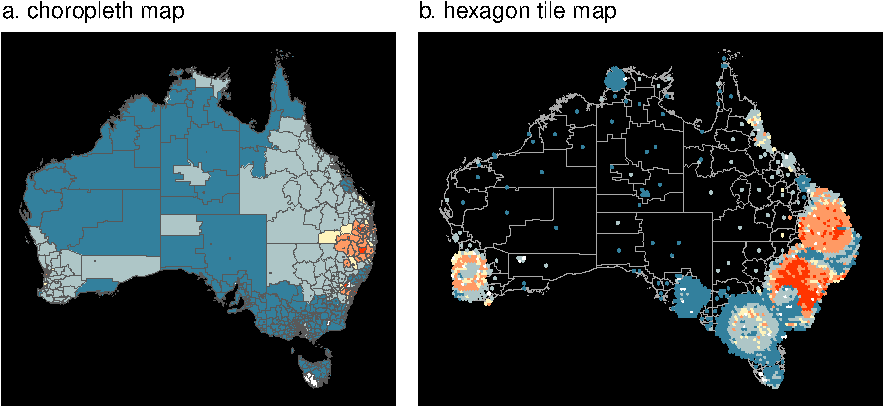
\includegraphics[width=1\linewidth,height=\textheight,keepaspectratio]{kobakian-cook-anzjs_files/figure-pdf/fig-thyroid-1.pdf}

}

\caption{\label{fig-thyroid}Thyroid cancer incidence among females
across the Statistical Areas of Australia at Level 2, displayed using a
choropleth (a) and a hexagon tile map (b). Blue indicates lower than
average, and red indicates higher than average incidence. The choropleth
suggests high incidence is clustered on the east coast but misses the
high incidence in Perth and a few locations in inner Melbourne visible
in the hexagon tile map.}

\end{figure}%

The choropleth map is an effective spatial display if the size of the
geographic units is relatively uniform. This is not the case for most
countries. Size heterogeneity in administrative units is particularly
extreme in Australia: most of the landscape of Australia is sparsely
settled, with the population densely clustered into the narrow coastal
strips. Figure~\ref{fig-thyroid} a shows the choropleth map of thyroid
cancer rates in Australia. The choropleth map focuses attention on the
geography, and for heterogeneously sized areas it presents a biased view
of the population related distribution of the statistic \citep{CBATCC}.
\emph{Land does not get cancer, people do} -- a more effective way to
communicate the spatial distributions of cancer statistics is needed
(sentiment motivated by \citet{monmonier2018how}).

A cartogram is a general solution for adequately displaying a
population-based statistic. It transforms the geographic map base to
reflect the population in the geographic region, while preserving some
aspects of the geographic location. There are several cartogram
algorithms \citep{ACTUC, CBATCC}; each involves shifting the boundaries
of geographic units, using the value of the statistic to increase or
decrease the area taken by the geographic unit on the map. The changes
to the boundaries result in cartograms that accurately communicate
population by map area for each of the geographic units but can result
in losing the familiar geographic information. For Australia, the
transformations warp the country so that it is no longer recognisable
(see \citet{KCR} for details).

Alternative algorithms make various trade offs between familiar shapes
and representation of geographic units. The non-contiguous cartogram
method \citep{NAC} keeps the shapes of geographic units intact, and
changes the size of the shape. This method disconnects areas creating
empty space on the display losing the continuity of the spatial display
of the statistic. The Dorling cartogram \citep{ACTUC} represents each
unit as a circle, sized according to the value of the statistic. The
neighbour relationships are mostly maintained by how the circles touch.
A similar approach was pioneered by \citet{RSCW}, using rectangles that
tile to align borders of neighbours \citep{CDWCS}. There have been
thorough reviews of the array of methods, as suitable for cancer atlas
displays \citep[e.g.][]{KCR, BCM}, and experiments demonstrating
cartograms to be more effective than choropleth maps \citep{KFIF}.

The hexagon tile map algorithm, automatically matches spatial regions to
their nearest hexagon tile, from a grid of tiles. It has the effect of
spreading out the inner city areas while maintaining the spatial
locations or regions in remote areas. The algorithm is available in the
R package, sugarbag \citep{sugarbag}. Figure~\ref{fig-thyroid} b shows
the hexagon tile map, where the map is coloured from low (blue) to high
(red). The inner city areas have expanded, making it possible to see the
cancer incidence in the small, densely populated areas. Remote regions
are represented by isolated hexagons, which is not ideal, but maintains
the spatial location of these data values. It is of interest to know how
well the spatial distribution patterns are seen from this display, in
comparison to how they are seen from the choropleth.

\subsection{Visual Inference}\label{visual-inference}

In order to assess the effectiveness of the hexagon tile map, the lineup
protocol \citep{BCHLLSW09, GIIV} from visual inference procedures is
employed. The approach mirrors classical statistical inference. The
procedures for doing a power comparison of competing plot designed,
outlined in \citet{GTPCCD}, are followed. It is the only current human
subjects testing protocol which quantitatively compares plot designs on
the basis of detection of structure relative to null distributions
\citep{VCH, VanderPlas2021Designing}. The premise for comparing two
designs is that the only difference between the two lineups is the plot
design, and hence difference in detection rate and time to detect is due
to the effectiveness of the plot design for differentiating between data
plot and null plots. The protocol has been used in to quantitatively
test plot designs numerous studies
\citep[e.g.][]{LHC, VH2016, KTV, RS2021}.

In classical statistical inference hypothesis testing is conducted by
comparing the value of a test statistic on a standard reference
distribution, computed assuming the null hypothesis is true. If the
value is extreme, the null hypothesis is rejected, because the test
statistic value is unlikely to have been so extreme if it was true. In
the lineup protocol, the plot plays the role of the test statistic, and
the data plot is embedded in a field of null plots. Defining the plot
using a grammar of graphics \citep{ggplot2} makes it a functional
mapping of the variables and thus, it can be considered to be a
statistic. With the same data, two different plots can be considered to
be competing statistics, one possibly a more powerful statistic than the
other.

Hypothesis testing with the lineup protocol requires human evaluation.
The human judge is required to identify the most different plot among
the field of plots. If this corresponds to the data plot -- the test
statistic -- the null hypothesis is rejected. It means that the data
plot is extreme relative to the reference distribution of null plots.

The null hypothesis is explicitly provided by the grammatical plot
description. For example, if a histogram is the map type being used, the
null might be that the underlying distribution of the data is a
Gaussian. Null data would be generated by simulating from a normal
model, with the same mean and standard deviation as the data. In
practice, the null hypothesis used is generic, such as \emph{there is NO
structure or a pattern in the plot}, and contrasted to an alternative
that there is structure.

The chance that an observer picks the data plot out of a lineup of size
\(m\) plots accidentally, if the null hypothesis is true is \(1/m\).
With \(K\) observers, the probability of \(k\) randomly choosing the
data plot, roughly follows a binomial distribution with \(p=1/m\).
Figure~\ref{fig-lineup} shows a lineup of the hexagon tile map, of size
\(m=12\). Plot 3 is the data plot, and the remaining 11 are plots of
null data. The supplementary materials contain all lineups used in the
study, including the corresponding lineup to this one made using
choropleth maps.

\begin{figure}

\centering{

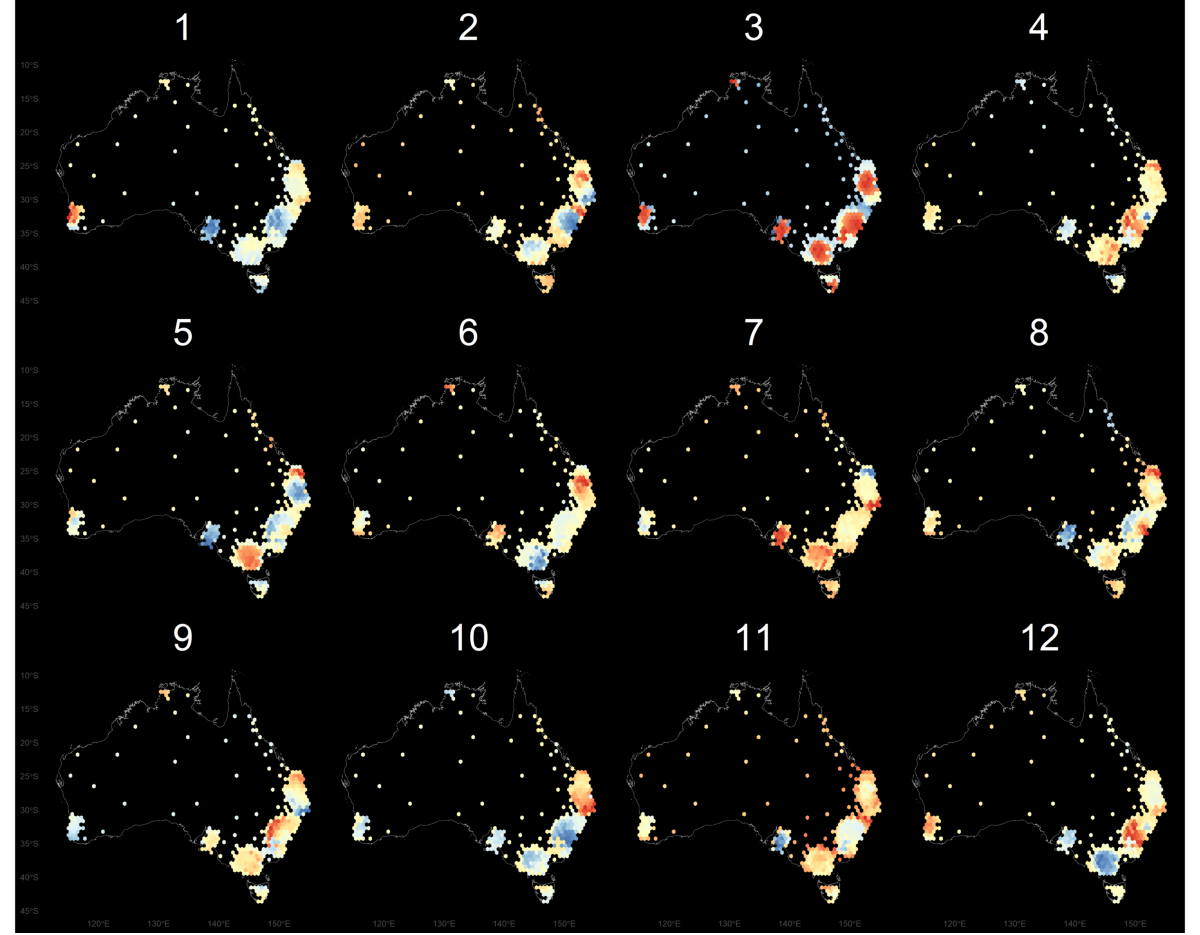
\includegraphics[width=1\linewidth,height=\textheight,keepaspectratio]{kobakian-cook-anzjs_files/figure-pdf/fig-lineup-1.pdf}

}

\caption{\label{fig-lineup}This lineup of twelve hexagon tile map
displays contains one map with a real population related structure
(location 3). The rest are null plots that contain only spatial
dependence.}

\end{figure}%

In order to determine the effectiveness of a type of display, this
probability is less relevant than the overall proportion of observers
who pick the data plot, \(k/K\). The power of the test statistic (data
plot) is provided by this proportion. Power in a statistical sense is
the ability of the statistic to \emph{produce a rejection} of the null
hypothesis, if it is indeed \emph{not true}. With the same data plotted
using two different displays, the display with the highest proportion of
people who choose the data plot would be considered to be the most
powerful statistic.

There are several practical considerations when deploying the lineup
protocol: (1) determining the appropriate null distribution to compute
null samples, (2) employing independent observers to conduct the
evaluations, (3) varying location of the data plot in a lineup, (4) how
many null sets to include in the lineup, (5) construction of all lineups
in the experiment (see \citet{VRCH}), (6) questions presented to
participants to solicit evaluations, in addition to the usual
experimental design issues. These are described in detail in the next
section.

\section{Methodology}\label{sec-methodology}

This study aims to answer two key questions around the presentation of
spatial distributions:

\begin{enumerate}
\def\labelenumi{\arabic{enumi}.}
\tightlist
\item
  Are spatial disease trends that impact highly populated small areas
  detected with higher accuracy, when viewed in a hexagon tile map?
\item
  Are people faster in detecting spatial disease trends that impact
  highly populated small areas when using a hexagon tile map?
\end{enumerate}

Additional considerations when completing this experimental task
included the difficulty experienced by participants and the certainty
they had in their decision.

Australia is used for the study, with Statistical Area 3 (SA3)
\citep{abs2016} as the geographic units. The results should apply
broadly to any other geographic areas of interest, if there are large
differences in area and population size.

\subsection{Experimental factors}\label{experimental-factors}

The primary factor in the experiment is the map type. The secondary
factor is a trend model. Three trend models were developed, one
mirroring a large spatial trend for which the choropleth would be
expected to do well, and two with differing level of inner city hot
spots. These latter two reflect the structure seen in the thyroid cancer
data (Figure~\ref{fig-thyroid}). This produces six treatment levels:

\begin{itemize}
\item
  Map type: \emph{Choropleth, Hexagon tile}
\item
  Trend:

  \begin{itemize}
  \tightlist
  \item
    \emph{NW-SE}: Large spatial trend running diagonally across
    Australia
  \item
    \emph{Three Cities}: Locations in three population centres
  \item
    \emph{All Cities}: Locations in all state and territory capitals
  \end{itemize}
\end{itemize}

Data is generated for each of the trend models, with four replicates,
and each displayed both as a choropleth and as a hexagon tile map, which
yields 12 data sets, and 24 data plots. This set of displays is divided
in half, providing two sets of 12 displays, Group A and Group B.
Participants were randomly allocated to Group A or B. Participants saw a
data set only once, either as a choropleth or as a hexagon tile map.
Figure~\ref{fig-exp-design} summarises the design and the allocation of
the displays.

\begin{figure}

\centering{

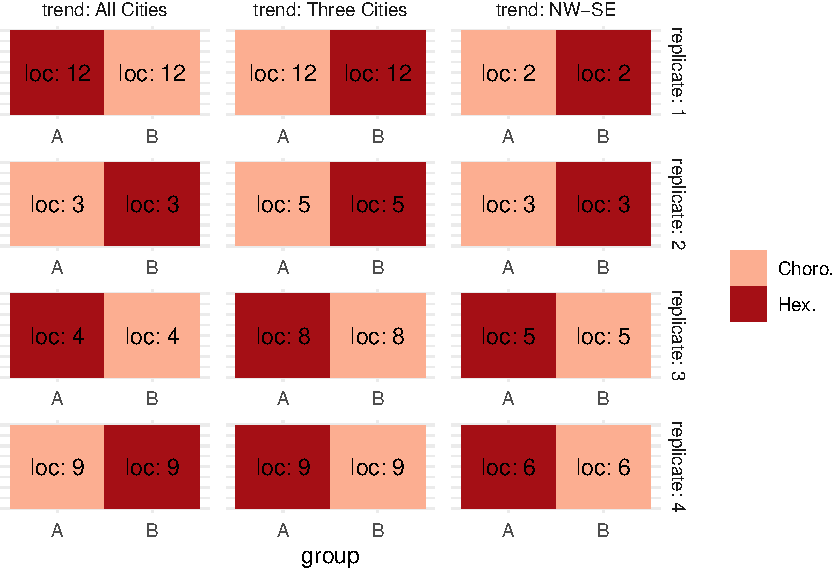
\includegraphics[width=1\linewidth,height=\textheight,keepaspectratio]{kobakian-cook-anzjs_files/figure-pdf/fig-exp-design-1.pdf}

}

\caption{\label{fig-exp-design}The experimental design used in the
study. Participants are allocated to with group A or B, to evaluate
either the choropleth or hexagon tile map lineup of each simulated data
set. The text `loc' refers to the location of the data plot in the
lineup.}

\end{figure}%

\subsection{Generating null data}\label{generating-null-data}

Null data needs to be data with no (interesting) structure. In most
scenarios, permutation is the main approach for generating null plots.
It is used to break association between variables, while maintaining
marginal distributions. This is too simple for spatial data. In spatial
data, a key feature is the spatial dependence or smoothness over the
landscape. To do something simple, like permute the values relative to
the geographic location would produce null plots which are too chaotic,
and the data plot will be recognisable for its smoothness rather than
any structure of interest.

For spatial data, null data is stationary data, where the mean, variance
and spatial dependence are constant over the geographic units.
Stationary data is specified by a variogram model \citep{POG}.
Simulating from a variogram model, where the spatial dependence is
specified, generates the stationary spatial data used for the null
plots. The parameters for the Gaussian model were sill=1, range=0.3 with
the variance generated by a standard normal distribution.

The R package \texttt{gstat} \citep{gstat} was used to simulate 144 null
sets, 12 data sets for each plot in a lineup, and 12 sets for 12
lineups. Simulating spatial dependence is difficult as discussed by
\citet{BDMSTW} as a blockage for using the lineup protocol for testing
map displays. Because the result from \texttt{gstat} was inadequate to
mirror the spatial dependence patterns results in the \citet{atlas},
each null set was further smoothed. This was done by averaging a small
number of spatial neighbours, approximating the methods described in
\citet{atlas-methods}.

\subsection{Generating lineups}\label{generating-lineups}

For each trend model, four real data displays were created by
manipulating the centroid values of each of the SA3 geographic units.
Each trend model is motivated by patterns observed in spatial data:
North West to South East (NW-SE) is a basic spatial trend across the
entire country, Three Cities is the existence of clusters of high
values, and All Cities is also clusters, but more of them. We would
expect that clusters pattern to be more visible with a hexagon tile map
but the large spatial trend to be more visible in the choropleth map.

The NW-SE distribution was created using a linear equation of the
centroid longitude and latitude values. The All Cities trend model was
created using the distance from the centroid of each geographic unit to
the closest capital city in Australia, calculated when creating the
hexagon tile map produced by the sugarbag \citep{sugarbag} package.
Two-thirds of SA3s (201/336) were considered greater capital city areas,
the values of these areas were increased to create red clusters. The
amount was chosen to make clusters around the cities visible, even in
the choropleth with careful inspection. A similar selection process was
applied to the Three Cities' trend model. However, for each of the four
replicates for the Three Cities trend, a random sample of capital cities
was taken from Sydney, Brisbane, Melbourne, Adelaide, Perth, and Hobart.
Only values of the areas nearest to the three cities were increased to
create clusters.

One of the plot locations (1-20) is chosen to embed the data plot, in
each of the four replicates, for the three trend models. These locations
were chosen by random sampling. Using random locations reduces the
chance that participants might inducing the location coincidentally.
Locations 1, 7, 10 and 11 were not in the sample. \citet{YMCCSG} used
the lineup protocol for a genomics study and similarly varied the the
location of the data plot in replicates of treatments. Their results
demonstrated that the actual location of the data plot didn't affect
performance. So we don't expect that the location affects results but
randomising locations among different lineups is to guard against
participants expecting the data plot to be in a particular location.

The lineup locations were the same for both map types, because each set
of lineup data was used to produce a choropleth map lineup and hexagon
tile map lineup. This ensures that performance on the two map types can
be directly compared. Lineups were grouped into A or B, so that a
participant saw only one version. Participants were assigned to group A
or B, randomly, and thus evaluated either the choropleth or the hexagon
tile map lineup. Because there were four replicates of each lineup, each
participant evaluated two choropleth and two hexagon tile map lineups,
for each trend model. This design is illustrated in
Figure~\ref{fig-exp-design}.

For each of the 144 individual maps, the values for each geographic area
were rescaled to create a similar colour scale from deep blue to dark
red within each map. This meant at least one geographic unit was
coloured dark blue, and at least one was red, in every map display of
every lineup.

For the geographic NW-SE distribution, this resulted in the smallest
values of the trend model (blue) occurring in Western Australia, the
North West of Australia, and the largest values of the trend model (red)
occurring in the South East. This resulted in Tasmania being coloured
completely red. For the other two trend types, clusters localised in the
cities appeared more red than the rest of Australia.

\subsection{Web application to collect
responses}\label{web-application-to-collect-responses}

The taipan \citep{taipan} package for R was used to create the survey
web application. This structure was altered to collect responses
regarding participants demographics and their survey responses. The
survey app contained three tabs. Participants were first asked for their
demographics their unique identifier and their consent to the responses
being used for analysis. The demographics collected included
participants' preferred pronoun, the highest level of education
achieved, their age range and whether they had lived in Australia.

After submitting these responses, the survey application switched to the
tab of lineups and associated questions. This allowed participants to
easily move through the twelve displays and provide their choice, reason
for their choice, and level of certainty.

When participants completed the twelve evaluations the survey
application triggered a data analysis script. This created a data set
with one row per evaluation. Containing the responses to the three
questions. The script also added the title of the image, which indicated
the type of map display, the type of distribution hidden in the lineup,
and the location of the data plot. It also calculated the time taken by
participant to view each lineup.

Each participant used the internet to access the survey, and data was
transferred by secure link from the web app to a Google sheet using the
\texttt{googlesheets} package tools \citep{sheets}.

\subsection{Participants}\label{participants}

Participants were recruited from the Figure Eight crowdsourcing platform
\citep{figeight} to evaluate lineups. The lineup protocol expects that
the participants are uninvolved judges with no prior knowledge of the
data, to avoid inadvertently affecting results. Potential participants
needed to have achieved level 2 or level 3 from prior work on the
platform, ensuring only participants with a good record on prior tasks
could provide evaluations. All participants were at least 18 years old.

Participants were allocated to either group A or group B when they
proceeded to the survey web application. There were 92 participants
involved in the study. All participants read introductory materials, and
were trained using three test displays, to orient them to the evaluation
task. All participants who completed the task were compensated \$AUD5
for their time, via the Figure Eight payment system.

A pilot study was conducted in the working group of the Econometrics and
Business Statistics Department of Monash University. This allowed us to
estimate the effect size, and thus decide on number of participants to
collect responses from.

\subsection{Data collection}\label{data-collection}

Each participant answered demographic questions and provided consent
before evaluating the lineups.

Demographics were collected regarding the study participants:

\begin{itemize}
\tightlist
\item
  Gender (female / male / other),
\item
  Education level achieved (high school / bachelors / masters /
  doctorate / other),
\item
  Age range (18-24 / 25-34 / 35-44 / 45-54 / 55+ / other)
\item
  Lived at least for one year in Australia (Yes / No )
\end{itemize}

Participants then moved to the evaluation phase. The set of images
differed for Group A and Group B. After being allocated to a group, each
individual was shown the 12 lineups in randomised order, and asked to
report:

\begin{itemize}
\tightlist
\item
  \textbf{Plot choice}: the number of the plot that they deemed to be
  most different from the others.
\item
  \textbf{Reason}: one of ``Clusters of colour'', ``Colour trend across
  the areas'', ``Big differences between neighbouring areas'', ``All
  areas have similar colours'' or ``None of these reasons''. Note
  providing restricted list of reasons rather than free text encourages
  a response because it is easy. The list needs to contain the primary
  expected reasons and other potential reasons need to be added so that
  it does not bias the participants' behaviour.
\item
  \textbf{Certainty}: how certain that their choice is different from
  the others, on a scale of 1-5.
\end{itemize}

on each of lineup. These responses are saved after entering.
Participants were expected to click the submit button on the final page.

\subsection{Analysis}\label{analysis}

\subsubsection{Data Cleaning}\label{data-cleaning}

Data is checked to ensure that survey responses collected for each
participants were only included once. Technically it is possible to
submit results more than once if the submit button is clicked multiple
times in short sequence. Participants who did not finish the evaluation
of all lineups or clicked through without providing their evaluation are
filtered.

\subsubsection{Descriptive statistics}\label{descriptive-statistics}

Basic descriptive statistics were computed for the different
experimental treatments. Basic plots summarising detection rates by map
type and trend model type, and feedback and demographic variables
against the different experimental design elements.

\subsubsection{Modelling}\label{modelling}

The likelihood of detecting the data plot in the lineup can be modelled
using a linear mixed effects model. The R \texttt{glmer()} function in
the \texttt{lme4} \citep{lme4} package implements generalised linear
mixed effect models. The model used includes the two main effects map
type and trend model, which gives the fixed effects model to be:

\[
\hat{y}_{ijk} \sim Bernoulli(p_{ijk})
\] with

\[
\text{logit}(p_{ijk}) = \mu_i + \tau_j + \delta_k + (\tau \delta)_{jk}
\]

where \(y_{ijk} = 0, 1\) represents whether subject \(i\) detected the
data plot (1) or did not (0), \(\mu_i, ~i=1, \dots n\) is the
subject-specific random intercept, \(n\) is the number of subjects,
\(\tau_j, ~j=1,2\) is the map type effect, \(\delta_k, ~k=1,2,3\) is the
trend model effect. The interaction between map type and trend model
allows for any map type effect to differ between trend models. As each
participant provides results from 12 lineups, this model can account for
each individual participants' abilities with the subject-specific random
intercept.

\section{Results}\label{sec-results}

A total of 1273 responses were collected from 97 participants. A small
number of participants, 7, were removed because they did not provide at
least 11 responses, or left more than 3 at the default value of 0. These
are participants that stopped early or clicked through without doing the
evaluation. Set A was evaluated by 39 participants, and 51 evaluated set
B. This resulted in 1080 evaluations, corresponding to 90 subjects, each
evaluating 12 lineups, that were analysed on accuracy and speed. The
certainty and reasons of subjects in their answers is also examined.

\subsection{Accuracy}\label{accuracy}

Figure~\ref{fig-detect-compare} displays the average detection rates for
the two types of plot separately for each trend model. Each trend model
was tested using four repetitions, evaluations on the same data set were
seen as either choropleths or hexagon tile maps by each group as
specified in Figure~\ref{fig-exp-design}; the detection rates for each
display are connected by a line segment. The Three Cities and All Cities
trend models shown in the hexagon tile map allowed viewers to detect the
data plot substantially more often than the choropleth counterparts. One
replicate for the All Cities group had similar detection rates for both
map types - the rate of detection using the choropleth map was much
higher than other replicates. Surprisingly, participants could also
detect the gradual spatial trend in the NW-SE group from the hexagon
tile map. We expected that the choropleth map would be superior for the
type of spatial pattern, but the data suggests the hexagon tile map
performs slightly better, or equally as well.

\begin{figure}

\centering{

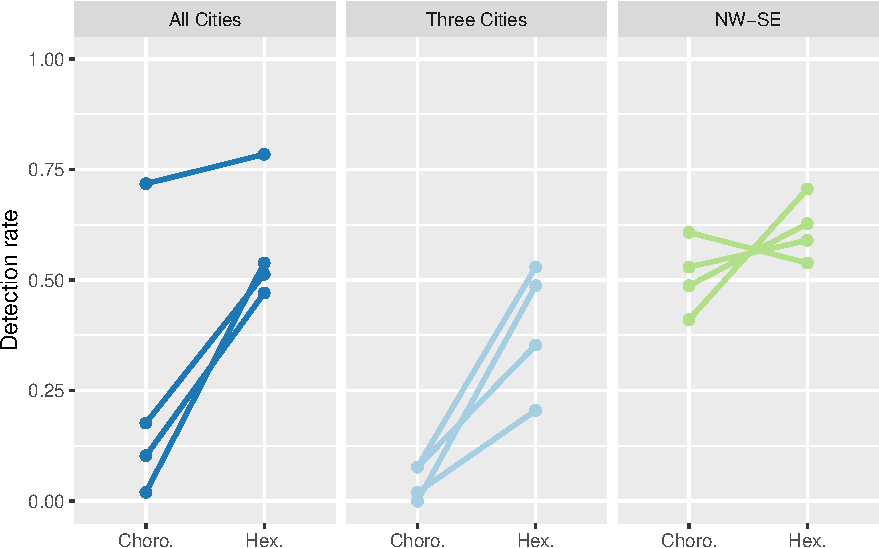
\includegraphics[width=1\linewidth,height=\textheight,keepaspectratio]{kobakian-cook-anzjs_files/figure-pdf/fig-detect-compare-1.pdf}

}

\caption{\label{fig-detect-compare}The detection rates achieved by
participants are contrasted when viewing the four replicates of the
three trend models. Each point shows the probability of detection for
the lineup display, the facets separate the trend models hidden in the
lineup. The points for the same data set shown in a choroleth or hexagon
tile map display are linked to show the difference in the detection
rate.}

\end{figure}%

\begin{table}

\caption{\label{tbl-detect-glmer1}Parameter estimates of the fitted
model fit for detection rate. All terms are statistically significant
(\(^{**}=0.01\), \(^{***}=0.001\)).}

\centering{

\begin{tabular}{rrlrr}
\toprule
Term & Est. & Std. Err. & P-val. & Sig.\\
\midrule
Intercept & -1.27 & 0.19 & 0.00 & $^{***}$\\
Hex. & 1.63 & 0.24 & 0.00 & $^{***}$\\
\addlinespace
Three Cities & -2.07 & 0.43 & 0.00 & $^{***}$\\
All Cities & 1.34 & 0.24 & 0.00 & $^{***}$\\
\addlinespace
Hex:Three Cities & 1.28 & 0.48 & 0.01 & $^{**}$\\
Hex:All Cities & -1.16 & 0.33 & 0.00 & $^{***}$\\
\bottomrule
\end{tabular}

}

\end{table}%

\begin{table}

\caption{\label{tbl-detect-prop}Model estimates for the proportion of
detection in each of the trend models (standard error). Note that
selecting the data plot by chance would produce a detection rate of
0.05.}

\centering{

\begin{tabular}{lccc}
\toprule
Map type & All Cities & Three Cities & NW-SE\\
\midrule
Choro. & 0.22 & 0.03 & 0.52\\
 & (0.03) & (0.01) & (0.04)\\
\addlinespace
Hex. & 0.59 & 0.39 & 0.63\\
 & (0.04) & (0.04) & (0.04)\\
\bottomrule
\end{tabular}

}

\end{table}%

Table~\ref{tbl-detect-glmer1} presents a summary of the generalised
linear mixed effects model, testing the effect of map type and trend
model on the detection rate. The results support the summary from
Figure~\ref{fig-detect-compare}. Overall, the hexagon tile map performs
marginally better than the choropleth for all trend models, and with
differing magnitudes of effects. The subject-specific random intercepts
have mean 0.3 and standard devation 0.55.

The estimated detection proportion from the model fit, computed using
the \texttt{emmeans} package \citep{Lenth2025} are shown in
Table~\ref{tbl-detect-prop}. For the All Cities trend participants were
about three times more likely to detect the cluster pattern with the
hexagon tile map than the choropleth. The Three Cities trend was
practically not detectable in the choropleth map. The dection rates were
more similar for the NW-SE trend, but slightly higher for the hexagon
tile map, which was a surprise. Note that, these detection rates are all
substantially higher than chance, except for the choropleth map on the
Three Cities. For a single evaluation the detection rate of the data
plot selected by chance is \(1/20=0.05\) because the lineups used in
this experiment had 20 plots. When designing an experiment like this it
is important to produce lineups that strike a balance between simple and
hard, so that there is a chance of discovering the effect of interest.
This experiment has managed to do this extremely well, which is a result
of pilot studies, careful null data generation, and power calculations
to determine appropriate sample size.

\begin{figure}

\centering{

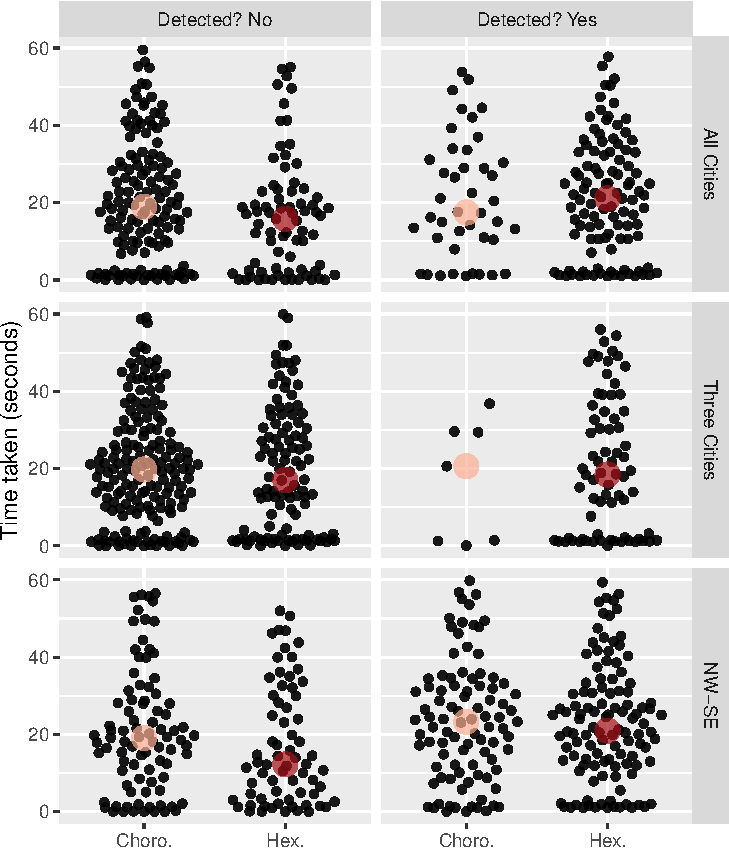
\includegraphics[width=1\linewidth,height=\textheight,keepaspectratio]{kobakian-cook-anzjs_files/figure-pdf/fig-beeswarm-1.pdf}

}

\caption{\label{fig-beeswarm}The distribution of the time taken
(seconds) to submit a response for each combination of trend, whether
the data plot was detected, and type of display, shown using
horizontally jittered dotplots. The coloured point indicates average
time taken for each map type. Although some participants take just a few
seconds per evaluation, and some take as much as 60 seconds, but there
is very little difference in time taken between map types.}

\end{figure}%

\subsection{Speed}\label{speed}

Figure~\ref{fig-beeswarm} shows horizontally jittered dot plots to
contrast the time taken by participants to evaluate each lineup facetted
by map type and trend model. Each dot is an evaluation. The time taken
to complete an evaluation ranged from fractions of a second to 60
seconds. The average time taken for type of display is shown as a large
coloured dot on each plot, and show there is little difference in the
average time taken to read a lineup made with either a choropleth or
hexagon tile map.

That some evaluations occurred within milliseconds is a little
surprising. Investigating whether this was related the 28 of 1080
evaluations where participants left the default choice of 0, and we find
it is not; most of these people took the routine time to examine, and
then left it at the default suggesting that they just could not pick one
as different. This is the same as a non-detect. On a per participant
basis, the average time per lineup over the 12 evaluations ranged
between 3.91 and 40.42 seconds. The correlation between average
detection rate and time taken across subjects 0.3 which is weakly
positive. This is similar to what we have found in other studies, some
subjects are especially fast and accurate in visual evaluation, and
conversely some subjects are quite slow but inaccurate.

\begin{figure}

\centering{

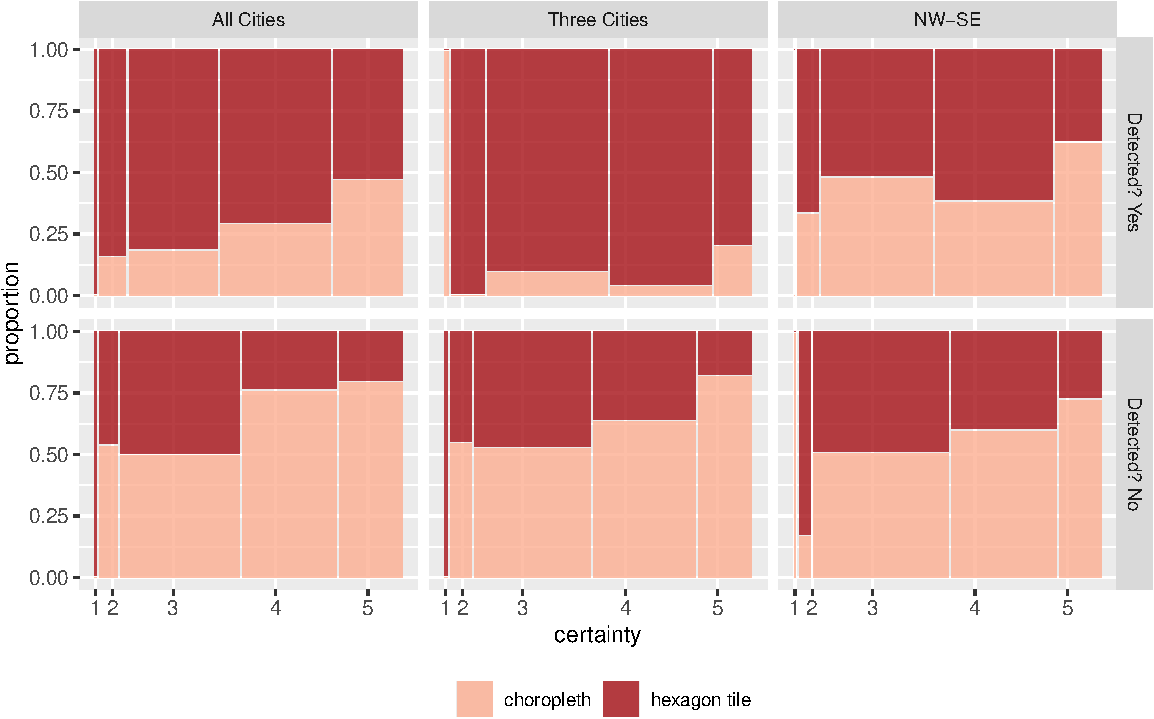
\includegraphics[width=1\linewidth,height=\textheight,keepaspectratio]{kobakian-cook-anzjs_files/figure-pdf/fig-certainty-1.pdf}

}

\caption{\label{fig-certainty}The distribution of certainty chosen by
participants when viewing hexagon tile map or choropleth displays, shown
as a mosaic plot, faceted by the trend model and whether the plot was
detected or not. At most trend models and whether the plot was detected
or not, participants were more likely to choose a high certainty when
evaluating a choropleth map.}

\end{figure}%

\subsection{Certainty}\label{certainty}

Participants provided their level of certainty regarding their choice
using a five point scale. Unlike the accuracy and speed of responses
that were derived during the data processing phase, this was a
subjective assessment by the participant prompted by the question: ``How
certain are you about your choice?''. Figure~\ref{fig-certainty} shows a
mosaic plot summarising how participants reported their certainty with
their decision. The plots are made separately for each combination of
trend models and whether the data plot was detected or not. Colour
indicates the type of map display. The proportion of subjects evaluating
the choropleth version increases as certainty increases, which suggests
overconfidence in their detection ability when using a choropleth map
display. Participants were less likely to be certain when their choice
was incorrect and they were viewing a hexagon tile map.

\subsection{Reason}\label{reason}

Table~\ref{tbl-reason} summarises the reasons that participants gave for
their choices: ``clusters'' = ``Clusters of colour'', ``trend'' =
``Colour trend across the areas'', ``consistent'' = ``All areas have
similar colours'', ``hotpots'' = ``Big differences between neighbouring
areas'', ``none'' = ``None of these reasons''. These proportions are
computed separately for each trend, map type and whether the participant
detected the data plot. With All Cities and Three Cities, when correct,
participants tended to select `consistent' with the choropleth, and
`clusters' with the hexagon tile map. With the NW-SE trend, `trend' was
primarily selected for the choropleth, but `clusters' was the primary
reason for the hexgon tile map. The primary reasons are similar when the
participant did not detect the data plot.

The results when the data plot was detected are as expected, but that
they are similar to the not detected group is interesting. It suggests
that with the choropleth people are trying to read contiguous patterns,
while the hexagon tile map is being read for pockets of differences.
This may be due the hexagon tile map being non-contiguous.

\begin{table}

\caption{\label{tbl-reason}Proportion of participants chose each reason
for their choice of plot, computed separately for each Trend and Map
Type level, and whether the data plot was detected. The primary reason
when participants were evaluating the choropleth map was `consistent' or
`trend', but for the hexagon tile map it was `clusters', when they
detected the data plot.}

\centering{

\begin{tabular}{lllrrrrr}
\toprule
Trend & Detect & Type & clusters & trend & consistent & hotspots & none\\
\midrule
All Cities & Yes & Choro. & 0.33 & 0.17 & 0.33 & 0.07 & 0.10\\
All Cities & Yes & Hex. & 0.42 & 0.33 & 0.04 & 0.13 & 0.08\\
\addlinespace
Three Cities & Yes & Choro. & 0.14 & 0.29 & 0.57 & 0.00 & 0.00\\
Three Cities & Yes & Hex. & 0.49 & 0.32 & 0.00 & 0.14 & 0.06\\
\addlinespace
NW-SE & Yes & Choro. & 0.34 & 0.40 & 0.02 & 0.16 & 0.08\\
NW-SE & Yes & Hex. & 0.50 & 0.29 & 0.11 & 0.05 & 0.05\\
\addlinespace
All Cities & No & Choro. & 0.36 & 0.41 & 0.09 & 0.08 & 0.07\\
All Cities & No & Hex. & 0.36 & 0.29 & 0.08 & 0.07 & 0.20\\
\addlinespace
Three Cities & No & Choro. & 0.31 & 0.43 & 0.07 & 0.10 & 0.09\\
Three Cities & No & Hex. & 0.39 & 0.31 & 0.06 & 0.10 & 0.14\\
\addlinespace
NW-SE & No & Choro. & 0.23 & 0.39 & 0.16 & 0.13 & 0.09\\
NW-SE & No & Hex. & 0.40 & 0.26 & 0.04 & 0.07 & 0.22\\
\bottomrule
\end{tabular}

}

\end{table}%

\subsection{Participant demographics}\label{participant-demographics}

Of the 90 participants, 66 were male, and 24 female. Most participants
(55) had a Bachelors degree, 13 had a Masters degree, and the remaining
22 had high school diplomas. The age distribution was 13, 36, 21, 11, 6
for age groups 18-24, 25-34, 35-44, 45-54, 55+, with 3 preferring not to
answer. Only 1 reported having lived in Australia. Note that, the
purpose of reporting these numbers is to illustrate the reasonable
variety of demographic background of participants. However, \$n=\$90 is
insufficient fit a model including this demographic information.
\citet{MHC} (published in 2025 but conducted in 2012) showed that there
is little difference in performance on lineup experiments between
demographic groups. \citet{VH2016} found that visual aptitude for
reading data plots was associated with math skills, but this study was
done on statistical plots of data, not maps. Assessing math ability
requires substantially more data collection, and does not necessarily
correlate with education level.

Summary statistics (not included here, but available in the analysis
code) show no differences in results between sets A and B in detection
rate or time taken. Similarly, detection rates and time taken vary
little across age, education and gender.

\section{Discussion}\label{discussion}

This study provides evidence that the hexagon tile map is superior to a
choropleth map for communicating population statistics, for Australia.
While the cartogram has been established as better than a choropleth
map, cartograms do not work for the vast disparity between population
density and geographic area in Australia. The hexagon tile map was
developed to provide a possible solution, and this study demonstrates
that it has potential.

The R package \texttt{sugarbag} can be used to generate a hexagon tile
map. It can be used for any spatial polygon data, so is applicable to
other countries or geographic areas.

One of the strengths but weaknesses of the hexagon tile map is that it
is non-contiguous. Large rural areas are represented by isolated
hexagons. This is why we expected that the hexagon tile map might not
work well to detect large-scale spatial trend (``NW-SE''). The primary
reason for producing the non-contiguous display was to preserve
geography sufficiently for the reader to easily recognise the location.
This is a strength, and allows a map of the country to be drawn
underneath the hexagons. It appears to not inhibit reading of the
spatial distribution based on this experiment. However, there is
considerable room for improving the algorithm and exploring some
variations. These might include increasing the size of isolated
hexagons, or collecting multiple hexagons together.

The manner in which hexagons are exploded out from the city centres is
another direction of research. Ideally, the location of the hexagons
should be close to their original location but this is hard to control
and measure. The current algorithm works sequentially to place hexagons,
radially from a provided centre. There are likely better optimisation
procedures that could impve the layout. For reading the spatial
distribution, this is less important, but if the hexagon tile map is
provided to users as an interactive tool, they will want to locate
themselves in the plot. If the hexagon is not close to the true location
it could be disconcerting.

Hexagon displays are growing in popularity. Two media outlets used
variations of the hexagon displays to communicate the 2025 Australian
federal election results
{[}\citet{abc-election2025};guardian-election2025{]}. Both are
effective, but have inadequacies. The Guardian preserves geography and
allows inner city results to be seen but the overall sense of the result
is skewed because the large rural areas dominate the display. The ABC's
contiguous hexagon tile map gives the correct sense of the final results
but loses the shape of Australia, and some hexagons are far from their
true location.

This experiment focused on comparing a new display, the hexagon tile
map, against the standard display, choropleth. There are other options
that could have been included in the study, such as the use of insets of
dense population areas along with the chorpleth map, or the use of
interactive graphics linking statistical charts with the choropleth.
Keeping the scope of the study small was important to understand whether
it was reasonable to recommend use of the hexagon tile map. Although we
only tested on the Australian geography, the results should hold for
other regions that have similarly disparities between population size
and geographic size.

We would recommend doing follow-up studies that allow deeper
understanding of how the different displays are read. For example, to
understand the differences in how people read the choropleth map and the
hexagon tile map as indicated by the different reasons given, could be
done using an eyetracking experiment. \citet{ZCHMR} is an example of
such an experiment where the manner in which people read lineups was
examined.

\section*{Acknowledgments}\label{acknowledgments}
\addcontentsline{toc}{section}{Acknowledgments}

The authors would like to thank the Australian Cancer Atlas team for
discussions regarding alternative spatial visualisations, and Professor
Kerrie Mengersen and Dr Earl Duncan for regular meetings filled with
suggestions and comments. Mitchell O'Hara-Wild was a co-developer of the
taipan \citep{taipan} R package for image tagging, used as the base for
the web app constructed to collect participant evaluations of lineups.
We are thankful for the NUMBATs (Non-Uniform Monash Business Analytics
Team) for participating in the pilot study that helped to assess the
experimental design and determine an appropriate sample size for the
study.

\section*{Supplementary materials and
reproducibility}\label{supplementary-materials-and-reproducibility}
\addcontentsline{toc}{section}{Supplementary materials and
reproducibility}

This document was written using quarto. This document contains the code
to produce the summaries, plots and additional checks in the paper. and
all the code to reproduce the analysis, and do additional checks can be
found on \href{https://github.com/srkobakian/experiment/paper}{GitHub}.
Supplementary materials have been included to discuss the survey
procedures and the lineups that were used. The full set of images can be
found here, too.

The supplementary material contains:

\begin{itemize}
\tightlist
\item
  Additional analysis of the experimental results
\item
  Survey procedure including training materials for the participants
\item
  24 lineups as images, that were used in the experiment
\item
  12 data sets used to construct the lineups
\end{itemize}

The analysis of the work was completed in R \citep{RCore} with the use
of the following packages:

\begin{itemize}
\tightlist
\item
  Document creation: quarto \citep{Allaire_Quarto_2025}, anzjs template
  \citep{quarto-anzjs}, knitr \citep{knitr}.
\item
  Lineup creation: nullabor \citep{nullabor}, gstat \citep{gstat}.
\item
  Data analysis: tidyverse \citep{tidyverse}, ggthemes \citep{ggthemes},
  RColorBrewer \citep{RColorBrewer}.
\item
  Plots: ggplot2 \citep{ggplot2}, cowplot \citep{cowplot}, png
  \citep{png}, ggbeeswarm \citep{ggbeeswarm}, ggmosaic \citep{ggmosaic}.
\item
  Modelling and summary presentation: lme4 \citep{lme4}, kableExtra
  \citep{kableExtra}.
\end{itemize}

\section*{Ethics Declaration}\label{ethics-declaration}
\addcontentsline{toc}{section}{Ethics Declaration}

Ethics approval for the online survey was granted by QUT's Ethics
Committee (Ethics Application Number: 1900000991). All applicants
provided informed consent in line with QUT regulations prior to
participating in this research.


\bibliography{paper.bib}



\end{document}
